% Q08 -- 1T DRAM cell STICK diagram (simplified, colour-coded layers).
% poly = red (WL gate), n-diffusion = green (access transistor), metal = blue (BL + cap plate),
% contacts = black squares. WL poly crossing the n-diffusion forms the access transistor.
\documentclass[border=10pt]{standalone}
\usepackage{tikz}
\begin{document}
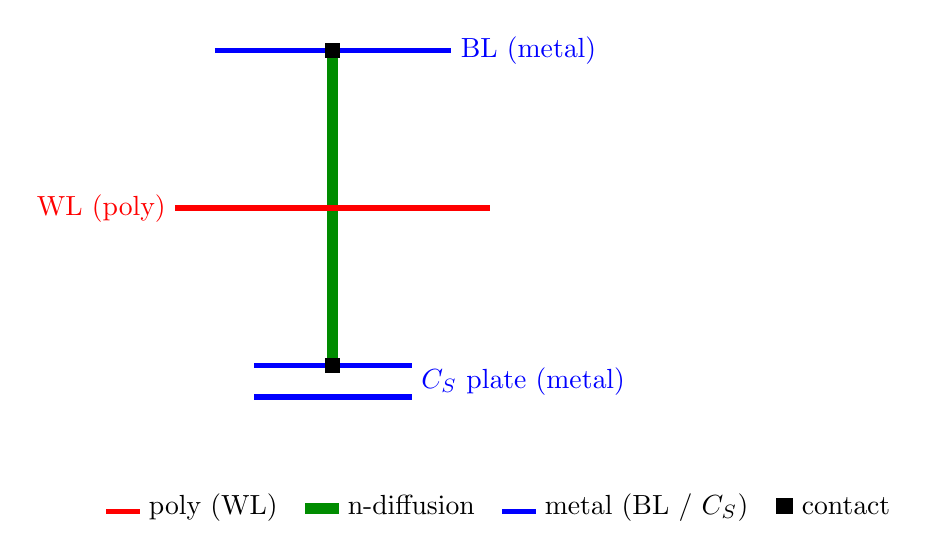
\begin{tikzpicture}[
  poly/.style={red, line width=2pt},
  ndiff/.style={green!55!black, line width=4pt},
  metal/.style={blue, line width=2pt},
  cont/.style={fill=black, draw=black, minimum size=5pt, inner sep=0pt}]
% n-diffusion (vertical strip = source/channel/drain of access nMOS)
\draw[ndiff] (3,1) -- (3,5);
% word line (poly) crossing the diffusion -> gate of access transistor
\draw[poly] (1,3) -- (5,3);
\node[left, red] at (1,3) {WL (poly)};
% bit line (metal) at top + contact to diffusion
\draw[metal] (1.5,5) -- (4.5,5);
\node[right, blue] at (4.5,5) {BL (metal)};
\node[cont] at (3,5) {};
% storage capacitor plate (metal) at bottom + contact to diffusion
\draw[metal] (2,1) -- (4,1);
\draw[metal] (2,0.6) -- (4,0.6);
\node[right, blue] at (4,0.8) {$C_S$ plate (metal)};
\node[cont] at (3,1) {};
% legend
\node[anchor=west, align=left] at (0,-0.8)
 {\textcolor{red}{$\rule{12pt}{2pt}$} poly (WL)\quad
  \textcolor{green!55!black}{$\rule{12pt}{4pt}$} n-diffusion\quad
  \textcolor{blue}{$\rule{12pt}{2pt}$} metal (BL / $C_S$)\quad
  \rule{6pt}{6pt}~contact};
\end{tikzpicture}
\end{document}
